In the following, a brief introduction to tensors, tensor networks, and tensor network algorithms is given. We start by defining the conventions and notation used in this thesis in Section \ref{sec:tensors_and_tensor_networks_conventions_and_notation}. In Section \ref{sec:tensors_and_tensor_networks_tensor_decompositions} we introduce important tensor decompositions that are used extensively in tensor network algorithms. In Section \ref{sec:tensors_and_tensor_networks_isometric_tensor_networks} we define isometric tensor networks and discuss their properties. Lastly, we give examples for physical states being represented in terms of isometric tensor networks, namely the popular Matrix Product States (MPS) in Section \ref{sec:tensors_and_tensor_networks_matrix_product_states} and the recently developed isometric tensor product states in 2D (isoTPS) in Section \ref{sec:tensors_and_tensor_networks_isometric_tensor_product_states_in_2D}.

\section{Conventions and Notation}
\label{sec:tensors_and_tensor_networks_conventions_and_notation}
For the purpose of this thesis we define a \textit{tensor} $T$ \textit{of rank} $n$ as an $n$-dimensional array of complex numbers
\begin{equation}
	\label{eq:general_tensor_rank_n}
	T \in \mathbb{C}^{\chi_1\times\chi_2\times\dots\times\chi_n}, \quad \chi_i \in \{1, 2, \dots\}
\end{equation}
with entries
\begin{equation}
	T_{i_1i_2\dots i_n} \in \mathbb{C}, \quad i_j \in \{1, 2, \dots, \chi_j\}.
\end{equation}
For example, a rank-0 tensor is a scalar, a rank-1 tensor is a vector, and a tensor of rank-2 is a matrix. It is convenient to use a diagrammatic notation, drawing tensors as shapes and tensor indices as lines (legs) emerging from these shapes. As an example we draw a few simple tensors in tensor diagram notation in Figure \figref{fig:basic_tensor_diagrams}. \par
\begin{figure}[h]
	\centering
	% Store largest image in a box
	\savebox{\largestimage}{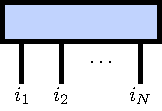
\includegraphics[scale=1]{figures/tikz/Tensor_Networks/basic_diagrams/basic_diagrams_d.pdf}}
	\subcaptionbox{\label{fig:basic_tensor_diagrams_scalar}}
	{%
		\raisebox{\dimexpr.5\ht\largestimage-.5\height}
		{%
			
\includegraphics[scale=1]{figures/tikz/Tensor_Networks/basic_diagrams/basic_diagrams_a.pdf}
		}
	}
	\quad\quad
	\subcaptionbox{\label{fig:basic_tensor_diagrams_vector}}
	{%
		\raisebox{\dimexpr.5\ht\largestimage-.5\height}
		{%
			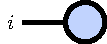
\includegraphics[scale=1]{figures/tikz/Tensor_Networks/basic_diagrams/basic_diagrams_b.pdf}
		}
	}
	\quad\quad
	\subcaptionbox{\label{fig:basic_tensor_diagrams_matrix}}
	{%
		\raisebox{\dimexpr.5\ht\largestimage-.5\height}
		{%
			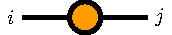
\includegraphics[scale=1]{figures/tikz/Tensor_Networks/basic_diagrams/basic_diagrams_c.pdf}
		}
	}
	\quad\quad
	\subcaptionbox{\label{fig:basic_tensor_diagrams_rank_n_tensor}}
	{%
		\usebox{\largestimage}
	}
\caption{Tensors of different ranks are shown in diagrammatic notation. (a) A scalar, (b) a vector, (c) a matrix, (d) a general tensor of rank $n$ as defined in Equation \eqref{eq:general_tensor_rank_n}.}
\label{fig:basic_tensor_diagrams}
\end{figure}
An \textit{index contraction} between two or more tensors is the linear operation that is performed by summing over a given set of indices. For example, the scalar product of two vectors $A\in\mathbb{C^\chi}$ and $B\in\mathbb{C^\chi}$,
\begin{equation}
	\label{eq:example_tensor_network_scalar_product}
	c = \sum_{\alpha=1}^{\chi}A_\alpha B_\alpha,\quad c\in\mathbb{C},
\end{equation}
and the matrix product of two matrices $A\in\mathbb{C}^{\chi_1\times\chi_2}$, $B\in\mathbb{C}^{\chi_2\times\chi_3}$,
\begin{equation}
	\label{eq:example_tensor_network_matrix_product}
	C_{ij} = \sum_{\alpha=1}^{\chi_2} A_{i\alpha} B_{\alpha j},\quad C\in\mathbb{C}^{\chi_1\times\chi_3}
\end{equation}
constitute index contractions. A more involved example is the index contraction of two rank-3 tensors $A\in\mathbb{C}^{\chi_1\times\chi_2\times\chi_3}$, $B\in\mathbb{C}^{\chi_2\times\chi_4\times\chi_5}$ and one rank-4 tensor $C\in\mathbb{C}^{\chi_3\times\chi_5\times\chi_6\times\chi_7}$, where we contract along the indices with dimension $\chi_2$, $\chi_3$ and $\chi_5$. The result is a rank-4 tensor $D\in\mathbb{C}^{\chi_1\times\chi_4\times\chi_6\times\chi_7}$:
\begin{equation}
	\label{eq:example_tensor_network_involved_network}
	D_{ijkl} = \sum_{\alpha=1}^{\chi_2} \sum_{\beta=1}^{\chi_3} \sum_{\gamma=1}^{\chi_5} A_{i \alpha \beta} B_{\alpha j\gamma} C_{\beta \gamma k l}.
\end{equation}
In tensor diagrams, index contractions are drawn by connecting the legs corresponding to contracted indices. Lines connecting two tensors are sometimes called \textit{bonds}, while indices not used in contractions are called \textit{open indices}. The \textit{bond dimension} $\chi_i$ denotes the number of different values an index $i$ can take. It is often more convenient to discuss tensor network algorithms in terms of diagrams than in terms of equations. \par
A \textit{tensor network} is defined as a set of tensors that is contracted in a specified way. We draw the tensor diagrams of the above equations in Figure \figref{fig:basic_tensor_network_diagrams}.\par
\begin{figure}[h]
	\centering
	% Store largest image in a box
	\savebox{\largestimage}{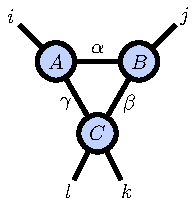
\includegraphics[scale=1]{figures/tikz/Tensor_Networks/basic_networks/basic_networks_c.pdf}}
	\subcaptionbox{\label{fig:basic_tensor_networks_matrix_vector_product}}
	{%
		\raisebox{\dimexpr.5\ht\largestimage-.5\height}
		{%
			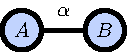
\includegraphics[scale=1]{figures/tikz/Tensor_Networks/basic_networks/basic_networks_a.pdf}
		}
	}
	\subcaptionbox{\label{fig:basic_tensor_networks_matrix_product}}
	{%
		\raisebox{\dimexpr.5\ht\largestimage-.5\height}
		{%
			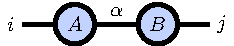
\includegraphics[scale=1]{figures/tikz/Tensor_Networks/basic_networks/basic_networks_b.pdf}
		}
	}
	\subcaptionbox{\label{fig:basic_tensor_networks_involved_contraction}}
	{%
		\usebox{\largestimage}
	}
	\caption{Tensor networks in diagrammatic notation. (a) Scalar product \eqref{eq:example_tensor_network_scalar_product}. (b) Matrix product \eqref{eq:example_tensor_network_matrix_product}. (c) More involved network consisting of three tensors \eqref{eq:example_tensor_network_involved_network}.}
	\label{fig:basic_tensor_network_diagrams}
\end{figure}
Because tensor contractions are linear, the order in which tensors are contracted does not change the result. However, the computational complexity does in general depend on the order of contractions and can thus be minimized by choosing the optimal contraction order. The computational complexity of a tensor contraction of two tensors is simply the product of all bond dimensions, where bond dimensions of contracted indices only appear in the product once. For example, the computational complexity of contracting tensors $B$ and $C$ from the contraction \eqref{eq:example_tensor_network_involved_network} scales as $\mathcal{O}(\chi_1\chi_2\chi_4\chi_5\chi_6\chi_7)$. \par
Given two normed vector spaces $V_1$ and $V_2$ with $\dim\left(V_1\right) = m$, $\dim\left(V_2\right) = n$, $m \le n$, an \textit{isometry} (sometimes also called \textit{semi-unitary}) is a linear, norm-preserving map $W: V_1 \rightarrow V_2$ from the smaller to the larger vector space. Each isometry can be represented by a $n\times m$ matrix $W$ fulfilling the \textit{isometry condition}
\begin{equation}
	\label{eq:isometry_condition_general}
	W^\dagger W = \id, \quad WW^\dagger = \mathbb{P},
\end{equation}
where $\mathbb{P} = \mathbb{P}^2$ is a projection. If $m = n$, it holds $\mathbb{P} = \id$ and $W$ is a \textit{unitary map}. An isometry tensor is a tensor that through grouping of indices and reshaping (i.e. matricization) becomes an isometry. In tensor network diagrams, we draw isometries by decorating lines with arrows. Following the convention of \cite{cite:isometric_tensor_network_states_in_two_dimensions, cite:efficient_simulation_of_dynamics_in_two_dimensional_quantum_spin_systems}, we denote the indices belonging to the larger vector space by incoming arrows and the indices belonging to the smaller vector space by outgoing arrows. Unitary tensors are decorated with bidirectional arrows on all indices, where the grouping must be inferred from the context. Ordinary tensors are drawn without arrows. Tensor diagrams for isometric and unitary tensors are shown in Figure \figref{fig:isometries_and_unitaries_diagrams}.\par
\begin{figure}[h]
	\centering
	\subcaptionbox{\label{fig:basic_isometries_isometric_matrix}}
	{%
		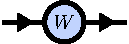
\includegraphics[scale=1]{figures/tikz/Tensor_Networks/basic_isometries/basic_isometries_a.pdf}
	}
	\par\bigskip
	\subcaptionbox{\label{fig:basic_isometries_unitary_matrix}}
	{%
	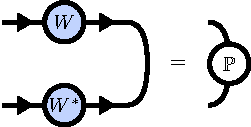
\includegraphics[scale=1]{figures/tikz/Tensor_Networks/basic_isometries/basic_isometries_c.pdf}
	}
	\par\bigskip
	\subcaptionbox{\label{fig:basic_isometries_isometric_tensor}}
	{%
		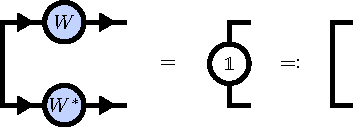
\includegraphics[scale=1]{figures/tikz/Tensor_Networks/basic_isometries/basic_isometries_b.pdf}
	}
	\caption{(a) A isometric matrix $W$ is depicted as a tensor diagram. The isometry condition \eqref{eq:isometry_condition_general} reduces contractions of $W$ with its adjoint to the identity matrix or to a projector $\mathbb{P}$. (b) A unitary matrix $U$ is drawn by using double arrows. For unitary matrices, the projector $\mathbb{P}$ is equal to the identity. (c) Isometric tensors of higher rank must fulfil the isometry condition by grouping of indices.}
	\label{fig:isometries_and_unitaries_diagrams}
\end{figure}
We lastly introduce an inner product for rank-$n$ tensors $A, B \in \mathbb{C}^{\chi_1\times\dots\times\chi_n}$, the \textit{Frobenius inner product}
\begin{equation}
	\label{eq:frobenius_inner_product}
	\left\langle A, B\right\rangle_\text{F} \coloneqq \sum_{\mu_1=1}^{\chi_1} \dots \sum_{\mu_n=1}^{\chi_n} A_{\mu_1\dots\mu_n}^*B_{\mu_1\dots\mu_n} = \Tr\left(A^\dagger B\right),
\end{equation}
where the last equality holds only if $n = 2$. The Frobenius inner product induces a norm, the \textit{Frobenius norm}
\begin{equation}
	\label{eq:frobenius_norm}
	\lVert A\rVert_\text{F} = \sqrt{\left\langle A, A\right\rangle_\text{F}},
\end{equation}
which can be used to define a measure of distance $\lVert A-B\rVert_\text{F}$ between tensors $A$ and $B$.

\newpage
\section{Tensor Decompositions}
\label{sec:tensors_and_tensor_networks_tensor_decompositions}
There are two decompositions that are used extensively in this thesis: The QR-decomposition and the Singular Value Decomposition. Both decompositions are matrix decompositions but can be applied to tensors as well by first grouping indices and reshaping to a matrix, applying the decomposition, and reshaping the result back to the original bond dimensions. \par
The \textit{reduced QR-decomposition} of a matrix $A \in \mathbb{C}^{n\times m}$ is the decomposition
\begin{equation}
	\label{eq:QR_decomposition_general}
	A = QR,
\end{equation}
where $Q\in\mathbb{C}^{n\times k}$ is an isometry, $R\in\mathbb{C}^{k\times m}$ is an upper triangular matrix and $k \coloneqq \min(n, m)$. The computational complexity of the QR decomposition scales as
\begin{equation}
	\label{eq:QR_decomposition_complexity}
	\mathcal{O}\left(n\cdot m\cdot\min(n, m)\right).
\end{equation}
A diagrammatic depiction of the QR decomposition \eqref{eq:QR_decomposition_general} is drawn in figure \figref{fig:tensor_decomposition_diagrams}(a). \par
The \textit{Singular Value Decomposition} (SVD) of a matrix $A \in \mathbb{C}^{n\times m}$ is the decomposition
\begin{equation}
	\label{eq:SVD_general}
	A = USV^\dagger,
\end{equation}
where $U\in\mathbb{C}^{n\times k}$ and $V\in\mathbb{C}^{m\times k}$ are isometries, $S\in\mathbb{R}^{k\times k}$ is a diagonal real matrix of \textit{singular values}, and $k \coloneqq \min(n, m)$. The computational complexity of the SVD is the same as for the QR decomposition \eqref{eq:QR_decomposition_complexity}. However, while the scaling is the same, the prefactors are lower for the QR decomposition in most implementations, meaning that the QR decomposition is faster in practice. Moreover, in contrast to the SVD, the QR decomposition allows for highly efficient implementations on graphics processing units (GPUs), which enables decompositions of large matrices to be carried out significantly faster and more power efficiently. Thus, whenever the singular values are not needed, the QR decomposition is preferred over the SVD. Figure \figref{fig:tensor_decomposition_diagrams} shows a tensor network diagram of the SVD \eqref{eq:SVD_general}. \par
An important property of the SVD is that it can be used to approximate a matrix $A$ by a matrix $\tilde{A}$ of lower rank $\chi < \min(m, n)$. This \textit{truncated SVD} can be performed by keeping only the largest $\chi < k$ singular values and omitting the corresponding columns of $U$ and $V$:
\begin{equation}
	\label{eq:truncated_SVD_general}
	A \approx \tilde{A} = \tilde{U}\tilde{S}\tilde{V},
\end{equation}
with isometries $\tilde{U}\in\mathbb{C}^{n\times\chi}$, $\tilde{V}\in\mathbb{C}^{m\times\chi}$ and real diagonal matrix $\tilde{S}\in\mathbb{C}^{\chi\times\chi}$. It can be shown \cite{cite:eckart_young_theorem} that the truncated SVD minimizes the distance $\lVert A - \tilde{A} \rVert_\text{F}$ between $A$ and $\tilde{A}$ under the constraint $\text{rank}(\tilde{A}) = \chi$. The truncated SVD is frequently used in tensor network algorithms to truncate tensors to a maximum bond dimension $\chi_\text{max}$. \par
\begin{figure}
	\centering
	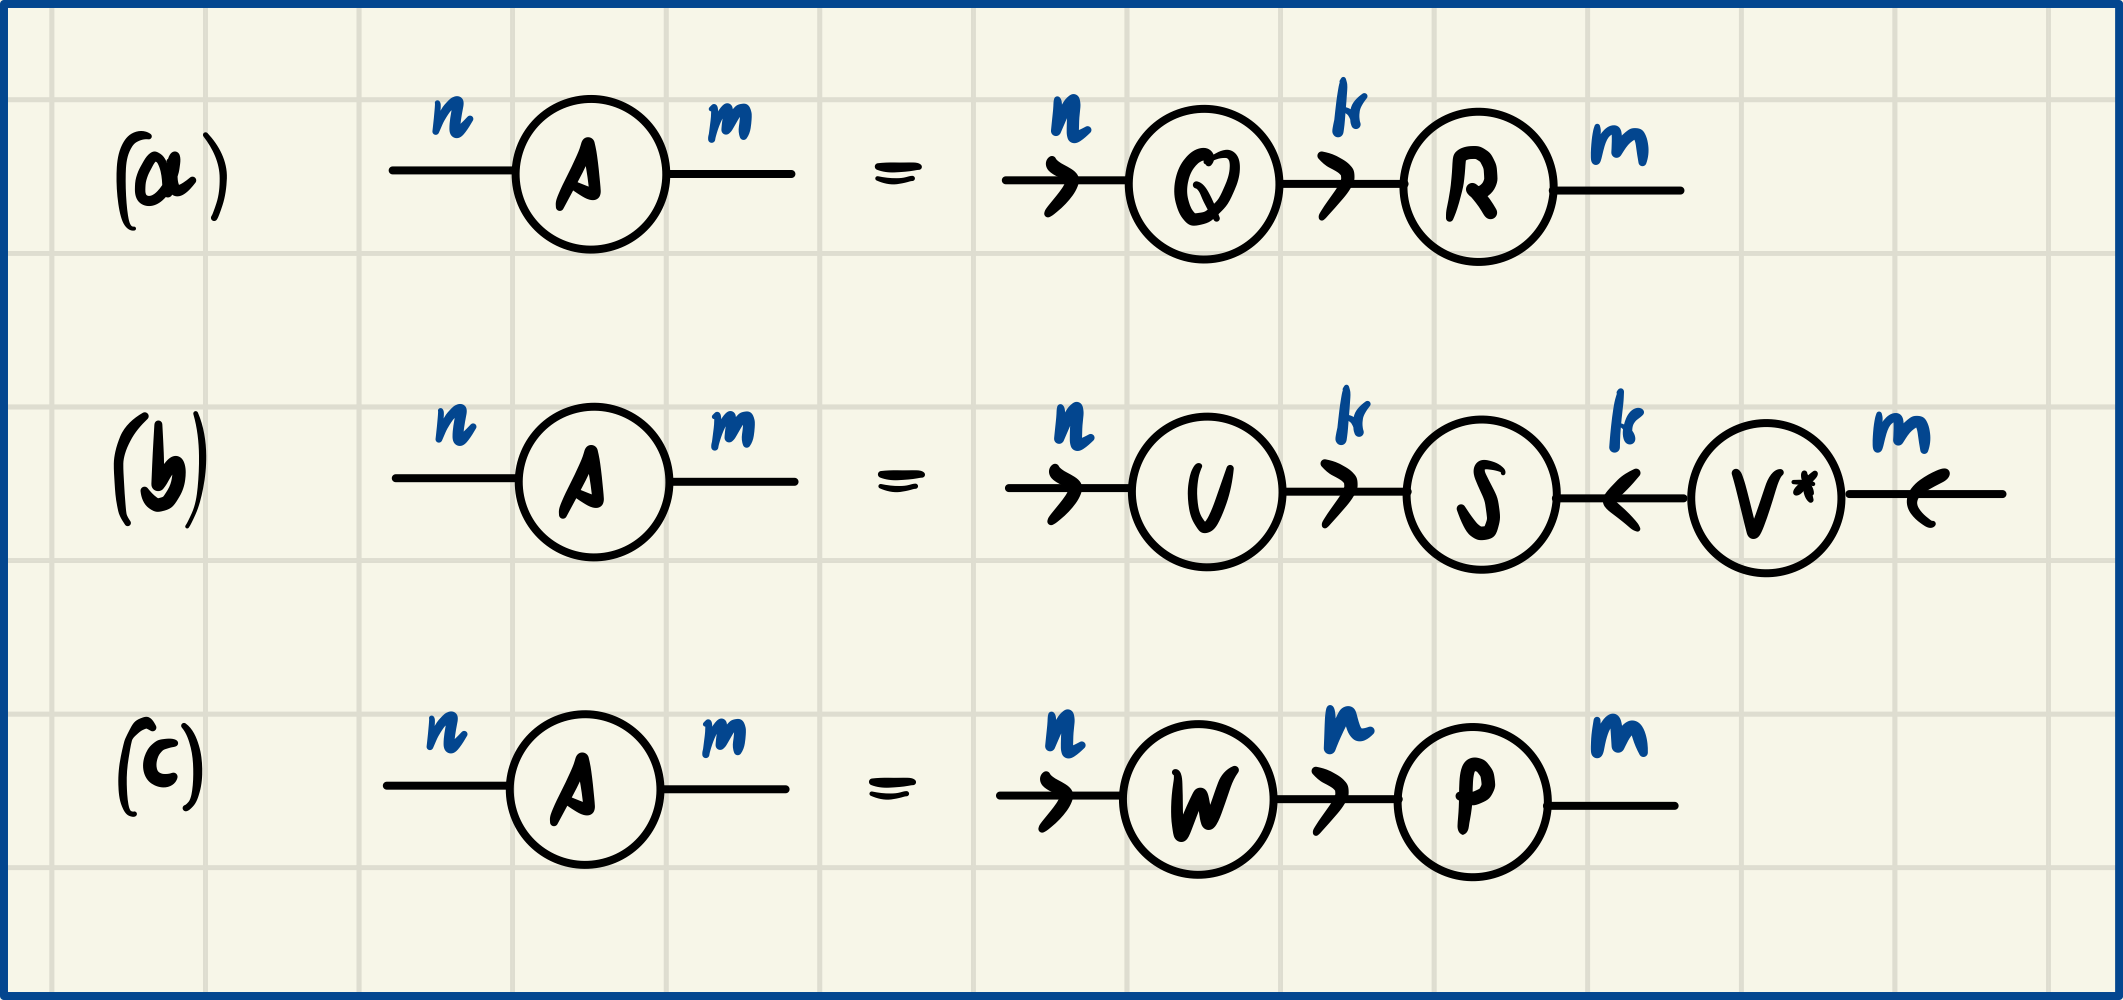
\includegraphics[width=0.8\textwidth]{figures/Tensor_Networks/tensor_decomposition_diagrams.jpeg}
	\caption{Different tensor decompositions are shown in tensor network diagram notation. The indices are decorated with bond dimensions. (a) QR decomposition \eqref{eq:QR_decomposition_general}. (b) Singular Value Decomposition \eqref{eq:SVD_general}}
	\label{fig:tensor_decomposition_diagrams}
\end{figure}
\todo{Discuss error of truncated SVD!}

\section{Isometric Tensor Networks}
\label{sec:tensors_and_tensor_networks_isometric_tensor_networks}
An isometric tensor network is a tensor network whose diagrams bonds can be consistently assigned with arrows. In particular we will look at finite tensor networks where the arrows do not form any loops. In such networks, all arrows point to a single tensor, the \textit{orthogonality center}. These networks have the very useful property that the error of local approximations around the orthogonality center can be computed locally, without contracting the full network. Let $\mathcal{N}$ be the tensor that is the result of contracting the full network, and let $\mathcal{M}$ be the tensor resulting from the contraction of a subregion of the network around the orthogonality center, where all arrows in the tensor network diagram point towards $\mathcal{M}$ (see Figure \figref{fig:isometric_tensor_network_N} for an example in tensor diagram notation). Let us now approximate the sub-network $\mathcal{M}$ by a different sub-network $\mathcal{M}^\prime$, which changes the contraction of the full network to $\mathcal{N}^\prime$ (see \figref{fig:isometric_tensor_network_N_prime}). We can compute the error $\varepsilon$ of this approximation as
\begin{equation}
\begin{split}
	\varepsilon^2 &= \lVert\mathcal{N}-\mathcal{N}^\prime\rVert^2_\text{F} \\
	&=
	\left\langle\mathcal{N}-\mathcal{N}^\prime, \mathcal{N}-\mathcal{N}^\prime\right\rangle_\text{F} \\
	&= \lVert\mathcal{N}\rVert_\text{F}^2 + \lVert\mathcal{N}^\prime\rVert_\text{F}^2 - 2\Re\left\langle\mathcal{N},\mathcal{N}^\prime\right\rangle_\text{F} \\
	&= \lVert\mathcal{M}\rVert_\text{F}^2 + \lVert\mathcal{M}^\prime\rVert_\text{F}^2 - 2\Re\left\langle\mathcal{M},\mathcal{M}^\prime\right\rangle_\text{F} \\
	&= \lVert\mathcal{M}-\mathcal{M}^\prime\rVert^2_\text{F},
\end{split}
\end{equation}
where in the fourth step we used the fact that all tensors outside of the sub-network satisfy the isometry condition. As an example, the contraction of $\langle\mathcal{N},\mathcal{N}^\prime\rangle_\text{F} = \langle\mathcal{M},\mathcal{M}^\prime\rangle_\text{F}$ is shown in Figure \figref{fig:isometric_tensor_network_norm_contraction}. As one can see, the computation of the error reduces to a contraction of the local sub-networks. This greatly simplifies the computation of optimal approximations of tensors especially for large networks because the full network does not need to be contracted. When the tensor network represents a quantum state, this also makes it very easy to compute local expectation values, as will become clear in the next section. This is because the computation of the overlap of the wave function can be simplified to a contraction of a local environment around the orthogonality center. Additionally, approximations made by the truncated SVD \ref{eq:truncated_SVD_general} are, when performed at the orthogonality center, globally optimal for isometric tensor networks, instead of only locally optimal for non-isometric tensor networks.
\begin{figure}
	\centering
	\subcaptionbox{\label{fig:isometric_tensor_network_N}}
	{%
		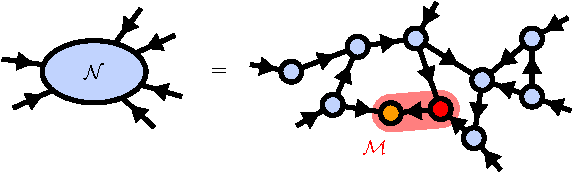
\includegraphics[scale=1]{figures/tikz/Tensor_Networks/contractions_of_isometric_tensor_networks/contractions_of_isometric_tensor_networks_a.pdf}
	}
	\par\bigskip
	\subcaptionbox{\label{fig:isometric_tensor_network_N_prime}}
	{%
		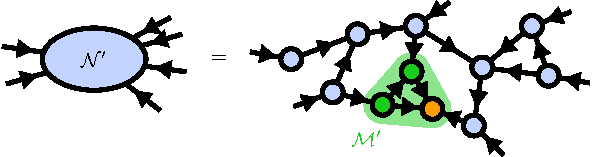
\includegraphics[scale=1]{figures/tikz/Tensor_Networks/contractions_of_isometric_tensor_networks/contractions_of_isometric_tensor_networks_b.pdf}
	}
	\par\bigskip
	\subcaptionbox{\label{fig:isometric_tensor_network_norm_contraction}}
	{%
		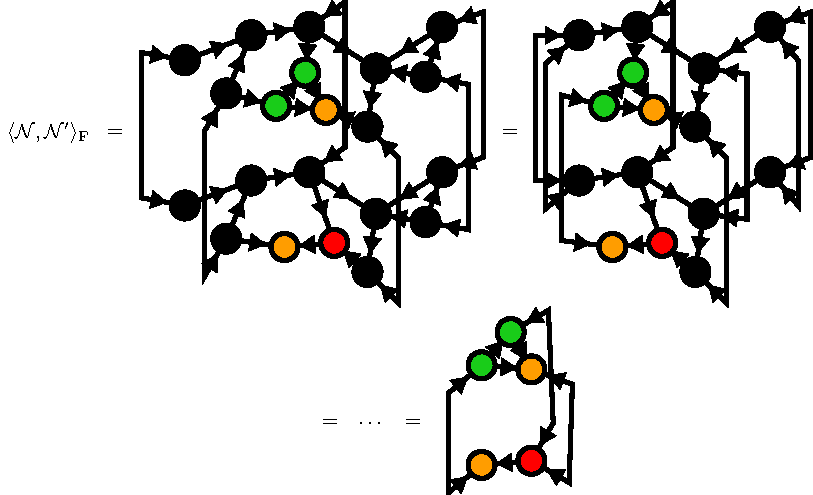
\includegraphics[scale=1]{figures/tikz/Tensor_Networks/contractions_of_isometric_tensor_networks/contractions_of_isometric_tensor_networks_c.pdf}
	}
	\caption{(a) An isometric tensor network $\mathcal{N}$ with the orthogonality center depicted in orange. The sub-network $\mathcal{M}$ is made up of all tensors in the red region. (b) The isometric tensor network $\mathcal{N}^\prime$ with an updated sub-network $\mathcal{M}^\prime$. (c) The computation of the inner product $\langle\mathcal{N},\mathcal{N}^\prime\rangle_\text{F}$ reduces to a contraction of the subregions $\langle\mathcal{M},\mathcal{M}^\prime\rangle_\text{F}$ because of the isometry condition. In the shown tensor network, the tensors of $\mathcal{N}^\prime$ are complex conjugated.}
	\label{fig:isometric_tensor_network_local_approximation}
\end{figure}

\newpage
\section{Matrix Product States (MPS)}
\label{sec:tensors_and_tensor_networks_matrix_product_states}
The Density Matrix Renormalization Group (DMRG) algorithm, a variational method over the class of Matrix Product States (MPS), has developed to be the de-facto standard for the numerical simulation of one-dimensional quantum systems. The success of this method is due to the remarkable ability of MPS to capture the area law entanglement characteristics of ground states of gapped Hamiltonians. Additionally, due to the elegant diagrammatic notation of tensor networks, new algorithms can be developed and discussed efficiently and intuitively. Applications of MPS include finding ground and thermal states, real and imaginary time evolution, and the computation of dynamical properties of lattice Hamiltonians. In the following, we give a brief introduction to MPS, for a more in-depth discussion see \cite{cite:DMRG_in_the_age_of_MPS, cite:practical_introduction_MPS_and_PEPS, cite:tenpy}. \par
The state of a quantum many-body system can be written as
\begin{equation}
	\ket{\Psi} = \sum_{i_1=1}^{d_1} \sum_{i_2=1}^{d_2} \cdots \sum_{i_N=1}^{d_N} \Psi_{i_1,i_2,\dots,i_N} \ket{i_1} \otimes \ket{i_2} \otimes \cdots \otimes \ket{i_N},
\end{equation}
where $N$ is the number of subsystems (e.g. lattice sites or particles), and $\left\{\ket{i_1} \otimes \ket{i_2} \otimes \dots \otimes \ket{i_N}\right\}$, $i_j = 0, \dots, d_j$ is a set of basis vectors of the full many-body Hilbert space
\begin{equation}
	\mathcal{H} = \bigotimes_{j=1}^{N} \mathcal{H}_j,
\end{equation}
with $\dim\left(\mathcal{H}_j\right) = d_j$ the dimension of the local Hilbert space of subsystem $j$. To simplify the notation, we will assume that the dimension of all local subsystems is the same, $d_j = d$. The $d^N$ complex numbers $\Psi_{i_1,i_2,\dots,i_N}$ fully describe the quantum many-body state, and one can think of $\Psi\in\mathbb{C}^{d\times\cdots\times d}$ as a tensor of rank $N$. However, due to the number of parameters scaling exponentially with system size, only very small system sizes are accessible computationally. One can proceed by writing $\Psi$ as a tensor network of tensors of lower rank. A \textit{Matrix Product State} (MPS) is constructed by introducing $N$ rank-3 tensors $T^{[n]}\in\mathbb{C}^{d\times \chi_{n-1}\times \chi_{n}}$ and contracting them in a chain as
\begin{equation}
	\label{eq:MPS_open_boundary_conditions_general_definition}
	\Psi_{i_1,i_2,\cdots,i_N} \coloneqq \sum_{\alpha_1=1}^{\chi_1} \sum_{\alpha_2=1}^{\chi_2}\dots\sum_{\alpha_{N-1}=1}^{\chi_{N-1}}T^{[1],i_1}_{1,\alpha_1} T^{[2],i_2}_{\alpha_1,\alpha_2} \cdots T^{[N],i_N}_{\alpha_{N-1},1},
\end{equation}
where we have written the indices $i_n$ as superscripts, such that the sums are performed only over subscripts. Note that in this notation the bond dimensions at the two ends of the chain are $\chi_0 = \chi_{N} = 1$, and we can interpret the tensors $T^{[1]}$ and $T^{[N]}$ as tensors of rank-2. Since the indices $i_n = 0, 1, \dots d$ represent the local physical degrees of freedom, they are sometimes referred to as \textit{physical indices}. The other indices are called \textit{virtual indices}. A tensor diagram of the MPS \eqref{eq:MPS_open_boundary_conditions_general_definition} is given in Figure \figref{fig:mps_general}.\par
\begin{figure}
	\centering
	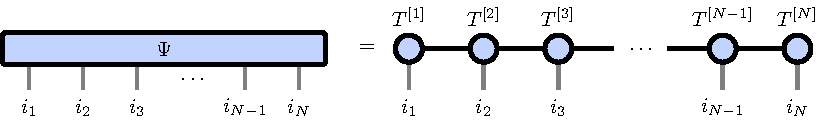
\includegraphics[scale=1]{figures/tikz/Tensor_Networks/mps_basic/mps_basic.pdf}
	\caption{Diagrammatic representation of the Matrix Product State \ref{eq:MPS_open_boundary_conditions_general_definition}.}
	\label{fig:mps_general}
\end{figure}
\begin{figure}
\centering
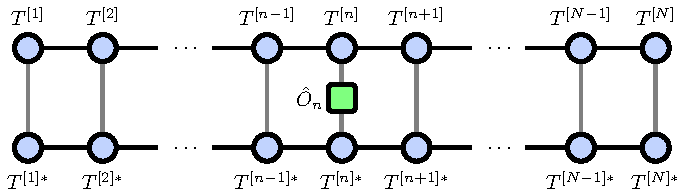
\includegraphics[scale=1]{figures/tikz/Tensor_Networks/mps_local_expectation_value/mps_local_expectation_value.pdf}
\caption{The computation of the expectation value of a local operator can be computed by contracting the MPS with its conjugate transpose, with the operator "sandwiched" in between.}
\label{fig:mps_local_expectation_value}
\end{figure}
An important property of MPS is the existence of a \textit{canonical form} as an isometric tensor network, where a single tensor $T^{[n]} \eqqcolon \Lambda^{[n]}$ is selected as the orthogonality center. One can bring an arbitrary MPS into this canonical form through successive QR-decompositions or SVDs, starting at the outer ends of the chain and isometrizing one tensor at a time, until the orthogonality center is reached \cite{cite:DMRG_in_the_age_of_MPS}. In Figure \figref{fig:mps_canonical_form_general_definition} an MPS in canonical form with the orthogonality center at subsystem $n$ is visualized in diagrammatic notation. We call tensors to the left of the orthogonality center $A^{[i]}$ and tensors to the right of the orthogonality center $B^{[i]}$. The canonical form greatly simplifies many operations on MPS and allows for the formulation of efficient algorithms, where many contractions reduce to identity due to the isometry condition \eqref{eq:isometry_condition_general}, see Figure \figref{fig:mps_left_isometry_condition} and Figure \figref{fig:mps_right_isometry_condition}. For example, the expectation value $\bra{\Psi}\hat{O}\ket{\Psi}$ of a one-site operator $\hat{O} \in \mathbb{C}^{d\times d}$ acting on site $n$ can for a general MPS be computed as
\begin{equation}
\begin{split}
	\label{eq:computation_of_expectation_value_MPS}
	\bra{\Psi}\hat{O}\ket{\Psi} &=\sum_{i_1,\dots,i_N,j_n=1}^{d}\Psi_{i_1,i_2,\dots,i_N} \Psi_{i_1,\dots,i_{n-1},j_n,i_{n+1},\dots,i_N}^* \bra{j_n}\hat{O} \ket{i_n} \\
	&= \sum_{i_1,\dots,i_N,j_n=1}^{d} \left(T^{[1],i_1}\cdots T^{[N],i_N}\right) \\
	&\quad\quad\quad\quad\quad\,\,\cdot\left(T^{[1],i_1*}\cdots T^{[n],j_n*} \cdots T^{[N],i_N*}\right)\cdot \hat{O}_{i_n,j_n},
\end{split}
\end{equation}
where the $T^{[n],i_n}$ are interpreted as matrices for $1 < n < N$ and as row/column vectors for $n = 1, N$ such that the product
\begin{equation}
	\left(T^{[1],i_1}\cdots T^{[N],i_N}\right)
\end{equation}
gives a scalar. The contraction \eqref{eq:computation_of_expectation_value_MPS} is visualized as a tensor diagram in Figure \figref{fig:mps_local_expectation_value}. Here the advantage of the diagrammatic notation becomes appearant: It is much easier to understand how tensors are contracted when expressing the contraction in terms of tensor network diagrams. The computational cost of computing the expectation value scales linear with the system size $\mathcal{O}\left(N\chi^3d\right)$, where $\chi$ is the maximum virtual bond dimension $\chi = \max\left\{\chi_1,\dots,\chi_N\right\}$. If the MPS is however given in canonical form with the orthogonality center at site $n$, the computation reduces to a contraction of only three tensors as can be seen in Figure \figref{fig:mps_local_expectation_value_canonical}, and the computational cost $\mathcal{O}\left(\chi^3d\right)$ becomes independent of system size. \par
\begin{figure}
	\centering
	\begin{minipage}{1.0\textwidth}
		\centering
		\subcaptionbox{\label{fig:mps_canonical_form_general_definition}}
		{%
			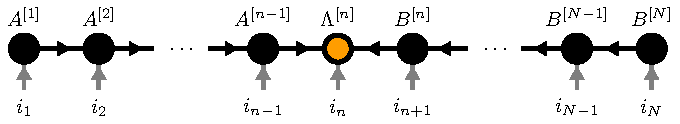
\includegraphics[scale=1]{figures/tikz/Tensor_Networks/mps_canonical_form/mps_canonical_form_a.pdf}
		}
	\end{minipage}
	\par\medskip
	\centering
	\subcaptionbox{\label{fig:mps_left_isometry_condition}}
	{%
		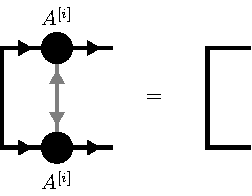
\includegraphics[scale=1]{figures/tikz/Tensor_Networks/mps_canonical_form/mps_canonical_form_b.pdf}
	}
	\quad\quad\quad\quad\quad
	\subcaptionbox{\label{fig:mps_right_isometry_condition}}
	{%
		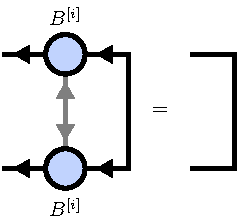
\includegraphics[scale=1]{figures/tikz/Tensor_Networks/mps_canonical_form/mps_canonical_form_c.pdf}
	}
	\caption{(a) Diagrammatic representation of an MPS in canonical form. (b) The left isometry condition. (c) The right isometry condition.}
	\label{fig:mps_canonical}
\end{figure}
\begin{figure}
	\centering
	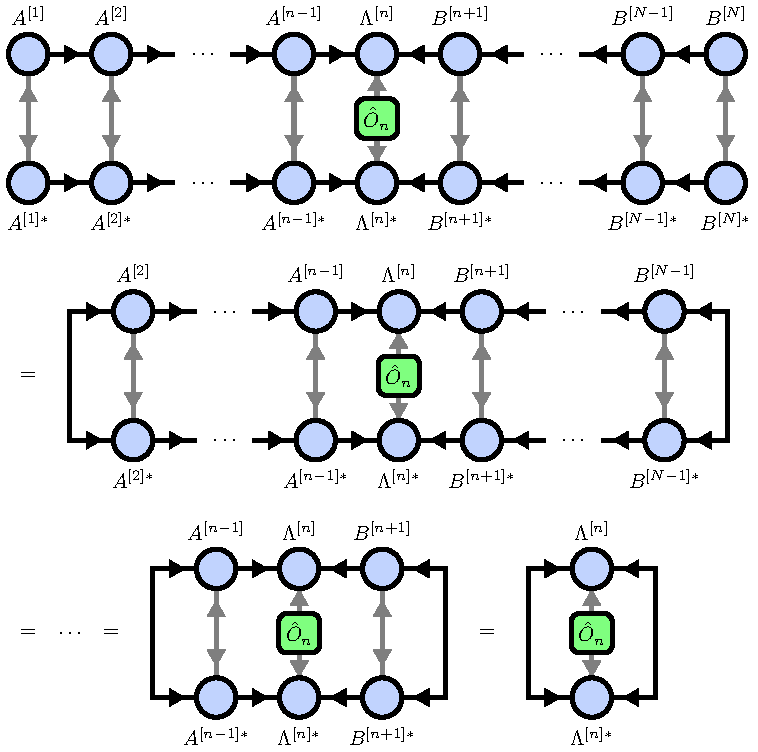
\includegraphics[scale=1.0]{figures/tikz/Tensor_Networks/mps_canonical_form_local_expectation_value/mps_canonical_form_local_expectation_value.pdf}
	\caption{If the MPS is in canonical form, the computation of the expectation value of a local operator can be simplified to a contraction of only three tensors using the isometry condition.}
	\label{fig:mps_local_expectation_value_canonical}
\end{figure}
\subsubsection*{\hspace{95pt}Approximating quantum states with MPS}
Until now, the MPS representation of $\ket{\Psi}$ is still exact. One can approximate an MPS by restricting the virtual bond dimension to a maximal bond dimension $\chi_n < \chi_\text{max}$. In this case, the number of parameters that need to be stored to describe the state is reduced from $\mathcal{O}\left(d^N\right)$ to $\mathcal{O}\left(N\chi_\text{max}^2 d\right)$. To arrive at this approximation, two neighbouring tensors can be contracted and split via a truncated SVD, keeping only the $\chi_\text{max}$ largest singular values. If the orthogonality center of the MPS is at one of the two tensors, this approximation is globally optimal as explained in Section \ref{sec:tensors_and_tensor_networks_isometric_tensor_networks}. Additionally, this SVD at the orthogonality center is related to the Schmidt decomposition of a bipartite system
\begin{equation}
	\ket{\Psi} = \sum_{\alpha=1}^{\chi_n} \lambda_\alpha \ket{\Psi^{[L]}_\alpha} \otimes \ket{\Psi^{[R]}_\alpha},
\end{equation}
where the chain is split into a left and right subsystem, grouping all indices to the left and right of the orthogonality center into orthogonal basis vectors $\ket{\Psi^{[L]}_\alpha}$ and $\ket{\Psi^{[R]}_\alpha}$ respectively. In this case, the Schmidt values $\lambda_\alpha >= 0$ coincide with the singular values \cite{cite:DMRG_in_the_age_of_MPS} and one can compute the Von-Neumann entanglement entropy
\begin{equation}
	S = -\sum_{\alpha=1}^{\chi_n} \lambda_\alpha^2 \log\left(\lambda_\alpha^2\right),
\end{equation}
quantifying the amount of entanglement between the left and right subsystem. If the state is normalized, it additionally holds
\begin{equation}
	\sum_{\alpha=1}^{\chi_n} \lambda_\alpha^2 = 1.
\end{equation}
Thus, how well an MPS of a given bond dimension $\chi_\text{max}$ is able to represent a given quantum state is highly dependent on the Schmidt spectrum $\left\{\lambda_\alpha\right\}$ at the different bipartitions of the chain. If the Schmidt values decrease exponentially, only an exponentially small part of the entanglement structure is truncated and the MPS is a good approximation for the original state. It can be shown \cite{cite:area_law_1D_proof, cite:area_laws_review} that for ground states of local, gapped, one dimensional Hamiltonians there holds an \textit{area law}: The entanglement entropy at arbitrary bipartitions of the chain is bounded by a constant
\begin{equation}
	S \le S_\text{max}, 
\end{equation}
where $S_\text{max}$ is independent of the system size. This is in contrast to the fact that the entanglement of states drawn randomly from the many-body Hilbert space on average exhibits \textit{volume law} scaling
\begin{equation}
	\mathbb{E}\left[S\right] > \min\left(N_L, N_R\right)\log(d),
\end{equation}
where $N_L$ and $N_R$ are the number of subsystems in the left and right bipartition. Hence, ground states of gapped Hamiltonians are very non-generic. Note that the constant $S_\text{max}$ scales with the correlation length of the system, which diverges when approaching critical points. \par
It is immediately clear that truncated MPS by construction exhibit area law entanglement scaling if the local subsystems that are represented by each tensor correspond to physical systems on a 1D chain. The maximal entanglement entropy for a bipartition can be reached when all Schmidt values are equal, i.e. $\lambda_\alpha = 1/\sqrt{\chi_n}$ for $\alpha = 1,\dots\chi_n$, and thus
\begin{equation}
	S \le \log\left(\chi_\text{max}\right)
\end{equation}
for arbitrary bipartitions of the chain. One can conclude that MPS are good approximations for ground states of gapped 1D Hamiltonians away from criticality. \par 
For completeness we note that the truncation of all bonds of an MPS is a highly non-linear optimization problem and the naive algorithm of truncating each bond with an SVD does in general not lead to a minimal error. A variational compression procedure can often be used to obtain a lower error at the same maximum bond dimension $\chi_\text{max}$ \cite{cite:DMRG_in_the_age_of_MPS}. \par
\subsubsection*{\hspace{162pt}Time evolution}
Many algorithms have been formulated in the language of MPS. Most notably, the Density Matrix Renormalization Group (DMRG) algorithm can be used for finding ground states of local lattice Hamiltonians \cite{cite:DMRG_in_the_age_of_MPS}. Time evolution of MPS can be performed with the the Time Evolving Block Decimation (TEBD) algorithm \cite{cite:efficient_simulation_of_1D_quantum_many_body_systems, cite:matrix_product_density_operators_simulation_of_finite_temperature_and_dissipative_systems} or the Time Dependant Variational Principle (TDVP) \cite{cite:time_dependent_variational_principle_for_quantum_lattices, cite:unifying_time_evolution_and_optimization_with_MPS}. In the following, we will briefly discuss TEBD, as this algorithm can be generalized easily to isometric tensor product states of higher dimension, which we will do in Section \ref{sec:YB_isoTPS_TEBD}. \par
Assume that we are given a quantum state $\ket{\Psi}$ in the form of an MPS and a Hamiltonian $\hat{H}$ that can be written as a sum of nearest-neighbour operators $\hat{h}^{[j,j+1]}$,
\begin{equation}
	\hat{H} = \sum_{j = 1}^{N-1} \hat{h}^{[j,j+1]}.
\end{equation}
According to the Schrödinger equation, the state $\ket{\Psi}$ can be evolved in time as
\begin{equation}
	\ket{\Psi(t)} = \hat{U}\left(t\right) \ket{\Psi} = e^{-it\hat{H}} \ket{\Psi},
\end{equation}
where we have set $\hbar = 1$. The time evolution operator $U(t)$ is in general very hard to compute and handle exactly. Thus, $U(t)$ is approximated using a \textit{Suzuki-Trotter decomposition}. We start by decomposing the time evolution into a series of $K$ small time steps $\Delta t = t/K$ as
\begin{equation}
	\hat{U}(t) = e^{-it\hat{H}} = \left(e^{-i\Delta t\hat{H}}\right)^K = \left(\hat{U}(\Delta t)\right)^K.
\end{equation}
Next, we split the Hamiltonian into terms acting on even and odd bonds
\begin{equation}
	\hat{H} = \sum_{j \text{ even}}\hat{h}^{[j, j+1]} + \sum_{j \text{ odd}}\hat{h}^{[j, j+1]} \eqqcolon \hat{H}_\text{even} + \hat{H}_\text{odd}.
\end{equation}
We can then use the \textit{Zassenhaus formula}
\begin{equation}
	e^{\varepsilon(\hat{A}+\hat{B})} = e^{\varepsilon \hat{A}} e^{\varepsilon \hat{B}} e^{-\frac{\varepsilon^2}{2}[\hat{A}, \hat{B}]} e^{\frac{\varepsilon^3}{6}\left(2[\hat{B},[\hat{A},\hat{B}]]+[\hat{A},[\hat{A},\hat{B}]]\right)} \dots
\end{equation}
which can be derived from the Baker-Campbell-Hausdorff formula, to approximate
\begin{equation}
	\label{eq:mps_first_order_tebd}
	\begin{split}
		\hat{U}(\Delta t) &= e^{-i\Delta t\left(\hat{H}_\text{even} + \hat{H}_\text{odd}\right)} = e^{-i\Delta t\hat{H}_\text{even}}e^{-i\Delta t\hat{H}_\text{odd}} + \mathcal{O}\left(\Delta t^2\right) \\
		&= \hat{U}^\text{TEBD1}(\Delta t) + \mathcal{O}\left(\Delta t^2\right).
	\end{split}
\end{equation}
This is called a Suzuki-Trotter decomposition of first order. Since operators acting on even bonds commute with each other, the exponential $e^{-i\Delta tH_\text{even}}$ factorizes,
\begin{equation}
	e^{-i\Delta t\hat{H}_\text{even}} = e^{-i\Delta t\sum_{j \text{ even}} \hat{h}^{[j, j+1]}} = \prod_{j \text{ even}} e^{-i\Delta t \hat{h}^{[j, j+1]}},
\end{equation}
and the same holds for the exponential $e^{-i\Delta t\hat{H}_\text{odd}}$. Each bond operator $\hat{U}^{[j, j+1]} \coloneqq e^{-i\Delta t \hat{h}^{[j, j+1]}}$ acting on the combined Hilbert space of sites $j$ and $j+1$ can be reshaped into a tensor of rank 4. The application of the operator $\hat{U}^\text{TEBD1}(\Delta t)$ to a state in MPS form can then be written as the tensor network in Figure \figref{fig:mps_tebd_first_order_overview}.
To perform a single TEBD iteration corresponding to a time evolution of $\Delta t$, we want to approximate this tensor network by a new MPS. This can be done by moving the orthogonality center from left to right, applying the bond operators $\hat{U}^{[j, j+1]}$ while keeping the MPS structure. The process of applying a single bond operator is shown in Figure \figref{fig:mps_tebd_first_order_applying_bond_op}. First, the orthogonality center is moved to site $j$. The two site tensors $\Lambda^{[j]}$ and $B^{[j+1]}$ are then contracted with the bond operator $\hat{U}^{[j, j+1]}$ into a single tensor $\theta$, which is subsequently split and truncated using an SVD. By sweeping twice across the MPS, first applying the bond operators on all even bonds and then the bond operators on all odd bonds, we perform a full TEBD iteration. There exist two sources of errors, the truncation error of the truncated SVD and the error of the Suzuki-Trotter decomposition. The truncation error can be controlled by choosing a larger bond dimension $\chi$, allowing the representation of more entanglement and thus the evolution to larger times. However, generally the amount of entanglement grows exponentially in time \cite{cite:DMRG_in_the_age_of_MPS}, necessitating an exponentially growing bond dimension and practically limiting the algorithm to small times. A smaller Suzuki-Trotter error can be achieved by choosing smaller time steps $\Delta t$ or by performing a higher-order Suzuki-Trotter decomposition. For example, a second order decomposition can be computed by symmetrizing two first-order decompositions of time step $\Delta t /2$ as
\begin{equation}
	\begin{split}
		\hat{U}(\Delta t) &= e^{-i\Delta t\left(\hat{H}_\text{even} + \hat{H}_\text{odd}\right)} = e^{-i\frac{\Delta t}{2}\hat{H}_\text{even}} e^{-i\Delta t \hat{H}_\text{odd}} e^{-i\frac{\Delta t}{2}\hat{H}_\text{even}} + \mathcal{O}\left(\Delta t^3\right)\\
		&= \hat{U}^\text{TEBD2}(\Delta t) + \mathcal{O}\left(\Delta t^3\right).
	\end{split}
\end{equation}
and can be applied to an MPS similarly as the first order decomposition. For higher order Suzuki-Trotter decompositions see \cite{cite:finding_exponential_product_formulas_of_higher_orders}.
\begin{figure}
	\centering
	\subcaptionbox{\label{fig:mps_tebd_first_order_overview}}
	{%
		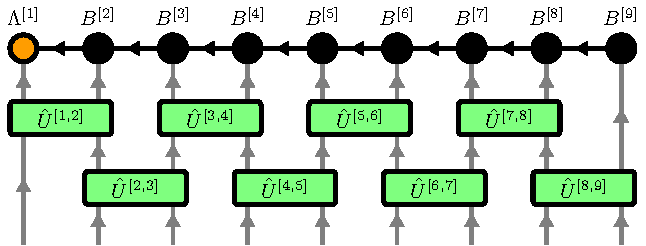
\includegraphics[scale=1]{figures/tikz/Tensor_Networks/mps_TEBD/mps_TEBD_a.pdf}
	}
	\par\medskip
	\subcaptionbox{\label{fig:mps_tebd_first_order_applying_bond_op}}
	{%
		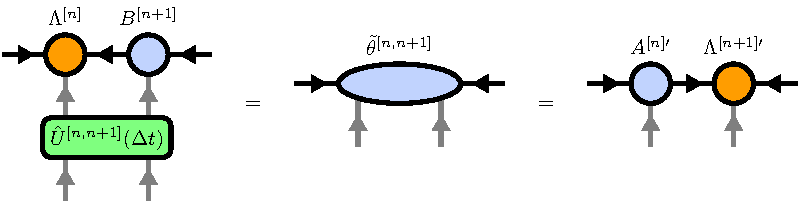
\includegraphics[scale=1]{figures/tikz/Tensor_Networks/mps_TEBD/mps_TEBD_b.pdf}
	}
	\caption{(a) An MPS can be approximately evolved by a time $\Delta t$ by applying the first order TEBD operator \eqref{eq:mps_first_order_tebd}, which is made up of bond operators acting first on all even and then on all odd bonds. (b) To apply a single bond operator $\hat{U}^{[n, n+1]}$, the two corresponding tensors $\Lambda^{[n]}$ and $B^{[n+1]}$ are contracted with the operator into a tensor $\theta^{[n,n+1]}$, which is then split using truncated SVD to obtain the updated tensors $A^{[n]\prime}$ and $\Lambda^{[n+1]^\prime}$.}
	\label{fig:mps_tebd_first_order}
\end{figure}

\section{Isometric Tensor Product States (isoTPS) in 2D}
\label{sec:tensors_and_tensor_networks_isometric_tensor_product_states_in_2D}
The natural generalization of MPS to higher dimensional lattices is given by \textit{Projected Entangled Pair States} (PEPS). A PEPS is constructed similar to a MPS by representing the local subsystem on each lattice site $i$ with the index $\sigma_i$ of a tensor $T_i^{\sigma_i}$ and connecting nearest-neighbour tensors with virtual bonds. The quantum state can then be written as
\begin{equation}
	\label{eq:PEPS_definition_general}
	\left|\Psi\right\rangle = \sum_{\sigma_1,\sigma_2,\dots,\sigma_N} \mathcal{C}\left(T_1^{\sigma_1}, T_2^{\sigma_2}, \dots, T_N^{\sigma_N}\right) \left|\sigma_1,\sigma_2,\dots,\sigma_N\right\rangle,
\end{equation}
where $\mathcal{C}(\dots)$ denotes the contraction of the full network along all virtual bonds. As an example, we draw a PEPS on a square lattice in figure \figref{fig:square_PEPS}. \par
\begin{figure}
	\centering
	\subcaptionbox{\label{fig:square_PEPS}}
	{%
		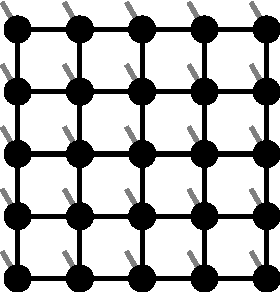
\includegraphics[scale=1]{figures/tikz/Tensor_Networks/isoTPS_structure/isoTPS_structure_a.pdf}
	}
	\quad\quad
	\subcaptionbox{\label{fig:square_isoTPS}}
	{%
		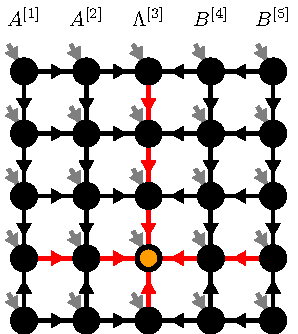
\includegraphics[scale=1]{figures/tikz/Tensor_Networks/isoTPS_structure/isoTPS_structure_b.pdf}
	}
	\caption{Tensor Networks representing two dimensional states on a square lattice. (a) A Projected Entangled Pair State (PEPS). (b) An isometric Tensor Product State (isoTPS). \todo{Include orthogonality center tensor}}
	\label{fig:square_PEPS_and_isoTPS}
\end{figure}
PEPS are able to efficiently represent area-law states in two and higher dimensions \cite{cite:practical_introduction_MPS_and_PEPS}. Remarkably, PEPS can even handle correlations decaying polynomially with separation distance \cite{cite:criticality_the_area_law_and_the_computational_power_of_PEPS}, whereas MPS can only handle exponentially decaying correlations. Polynomially decaying correlations are characteristic for critical points. \par
Unfortunately, it is not generally possible to bring a PEPS into an exact canonical form due to the presence of closed loops. Thus, already the computation of local expectation values scales exponentially with system size and can in practice be only done approximately, e.g. using the boundary MPS method \cite{cite:practical_introduction_MPS_and_PEPS} or corner transfer matrices \cite{cite:CTMRG}. Moreover, algorithms for ground state search and time evolution have computational costs scaling with high powers of the bond dimension. For example the cost of a full update TEBD or DMRG iteration is dominated by the contraction of an effective environment, scaling as $\mathcal{O}\left(D^{10}\right)$ \cite{cite:unifying_PEPS_contractions}. \par
Recently, the new class of \textit{isometric Tensor Product States} (isoTPS) has been introduced \cite{cite:isometric_tensor_network_states_in_two_dimensions, cite:conversion_of_PEPS_into_a_canonical_form, cite:DMRG_approach_to_optimizing_2D_tensor_networks}, generalizing the canonical form of MPS to higher dimensions by enforcing isometry constraints. This allows for efficient computation of local expectation values and greatly lowers the cost of some algorithms. The downside to this approach is that the set of states representable by isoTPS is smaller than the set of state representable by PEPS. It is thus an interesting question to ask which kinds of states and, more generally, which kinds of quantum phases can still be represented by isoTPS. \par
In the following, we will give a brief introduction to the isoTPS defined in \cite{cite:isometric_tensor_network_states_in_two_dimensions} and discuss their properties. A two-dimensional isoTPS on the square lattice is constructed by enforcing the isometry conditions shown in figure \figref{fig:square_isoTPS}. All isometries are chosen in such a way that all arrows point towards a special row and column, called the \textit{orthogonality hypersurface} of the isoTPS. The term "hypersurface" is chosen in anticipation of a generalization to higher dimensions. Because of the isometry condition, one can think of the contractions of each of the four regions outside the orthogonality hypersurface as orthogonal boundary maps \cite{cite:efficient_simulation_of_dynamics_in_two_dimensional_quantum_spin_systems}. The single tensor with only incoming arrows is called the \textit{orthogonality center}. local expectation values of operators acting in the vicinity of the orthogonality center can be computed efficiently because most contractions reduce to identity, similar to the computation of local expectation values in MPS (see figure \figref{fig:mps_local_expectation_value_canonical}). The orthogonality center can be moved along the orthogonality hypersurface simply and exactly using a QR-decomposition as shown in figure \figref{fig:isoTPS_moving_ortho_center}. \par
\begin{figure}
	\centering
	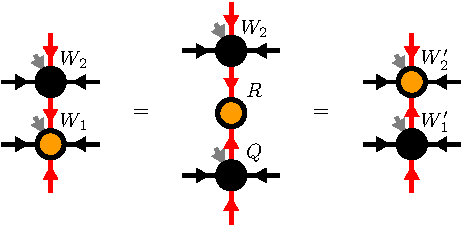
\includegraphics[scale=1]{figures/tikz/Tensor_Networks/isoTPS_moving_ortho_center/isoTPS_moving_ortho_center.pdf}
	\caption{Moving the orthogonality center and the orthogonality hyper surface around is a central problem in isoTPS applications. (a) Moving the orthogonality center along the orthogonality hypersurface can be done easily via QR-decompositions. (b) An orthogonality column can be moved by first solving equation \eqref{eq:isoTPS_moving_ortho_surface_auxillary_formulation} variationally and then absorbing $\Lambda$ into $B_{l+1}$ via the standard MPO-MPS multiplication and MPS compression algorithms.}
	\label{fig:isoTPS_moving_ortho_center}
\end{figure}
\begin{figure}
	\centering
	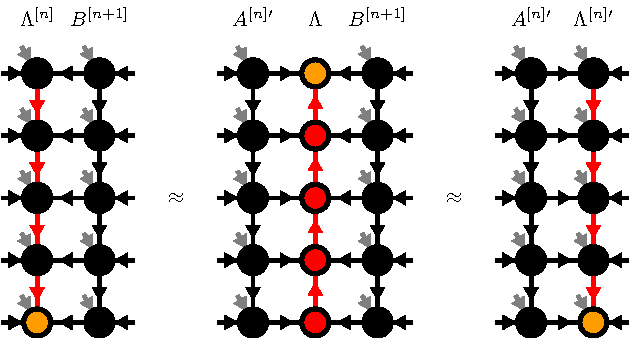
\includegraphics[scale=1]{figures/tikz/Tensor_Networks/isoTPS_moving_ortho_surface/isoTPS_moving_ortho_surface.pdf}
	\caption{The orthogonality hypersurface can be moved to the right by first solving equation \eqref{eq:isoTPS_moving_ortho_surface_auxillary_formulation} variationally and then absorbing $\Lambda$ into $B^{[n+1]}$ via the standard MPO-MPS multiplication and MPS compression algorithms.}
	\label{fig:isoTPS_moving_ortho_column}
\end{figure}
Moving the orthogonality surface is a harder problem, which in general can only be done approximately. In analogy to MPS and as shown in figure \figref{fig:square_isoTPS}, we call columns left of the orthogonality hypersurface $A_l$ and tensors right of the orthogonality hypersurface $B_l$, with $l = 1,2,\dots,L$ and $L$ the linear system size. Moving the orthogonality hypersurface $\Lambda_l$ one column to the right can be expressed as solving the problem
\begin{equation}
	\label{eq:isoTPS_moving_ortho_surface_general}
	\Lambda_l B_{l+1} = A_l \Lambda_{l+1},
\end{equation}
where the notation $\Lambda_l B_{l+1}$ means the contraction of columns $\Lambda_l$ and $B_{l+1}$ along their connecting bonds. Instead of \eqref{eq:isoTPS_moving_ortho_surface_general}, one can solve the simpler auxillary problem
\begin{equation}
	\label{eq:isoTPS_moving_ortho_surface_auxillary_formulation}
	\Lambda_l = A^l \Lambda,
\end{equation}
where $\Lambda$ is a column of tensors with no physical indices, as shown in figure \figref{fig:isoTPS_moving_ortho_column}. This column can then be absorbed into $B_{l+1}$ via the standard algorithm of applying an MPO to an MPS and subsequent MPS compression \cite{cite:DMRG_in_the_age_of_MPS}. One can variationally solve problem \eqref{eq:isoTPS_moving_ortho_surface_auxillary_formulation} by minimizing the distance $\left\lvert\Lambda_l-A_l\Lambda\right\rvert$, sweeping back and forth through the tensors while respecting the isometry condition.\todo{Maybe reference Evenbly-Vidal here?}
\begin{figure}
	\centering
	\subcaptionbox{\label{fig:Moses_move}}
	{%
		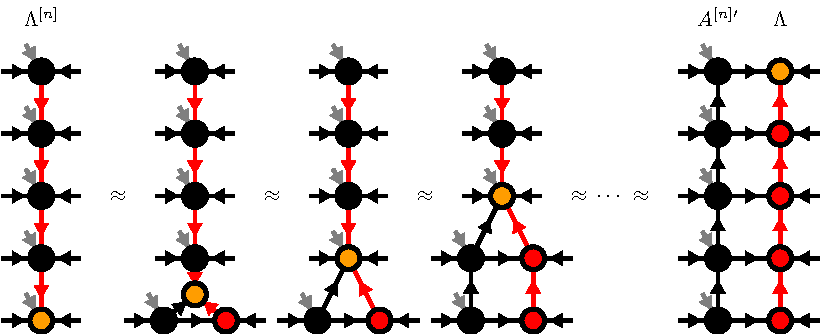
\includegraphics[scale=1]{figures/tikz/Tensor_Networks/isoTPS_MM/isoTPS_MM_a.pdf}
	}
	\subcaptionbox{\label{fig:tripartite_decomposition}}
	{%
		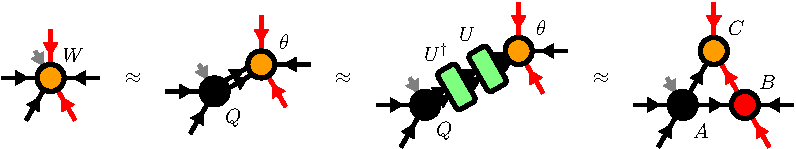
\includegraphics[scale=1]{figures/tikz/Tensor_Networks/isoTPS_MM/isoTPS_MM_b.pdf}
		
	}
	\caption{(a) The Moses Move (MM) splits the column $\Lambda_l$ into $A_l$ and $\Lambda$ via a single unzipping sweep of tripartite decompositions. (b) Tripartite decomposition of the tensor $W$ as explained in the text.}
	\label{fig:Moses_move_and_tripartite_decomposition}
\end{figure}
It is however found in \cite{cite:isometric_tensor_network_states_in_two_dimensions} that a single unzipping sweep, called the \textit{Moses Move} (MM), provides a solution very close to the variational one whilst being far quicker. The MM can also be used as a good initialization for the variational algorithm. We sketch the MM in figure \figref{fig:Moses_move}. We start from the bottom of the orthogonality hypersurface column and split the tensors one after the other using a tripartite decomposition. A single tripartite decomposition of a tensor $W$ is shown in figure \figref{fig:tripartite_decomposition}. First, $W$ is split into two tensors $A$ and $B$ via a truncated SVD $W = U(SV) = AB$ with $A$ an isometry. The bond connecting A and B is reshaped into two bonds. Next, it is important to note that the full contraction is invariant under the insertion of a unitary and its conjugate transpose, $AB = (AU^\dagger)(UB)$, with $(AU^\dagger)$ still satisfying the isometry condition. This degree of freedom can be used to \textit{disentangle} the tensor $B$ along the direction of the red bonds. Accordingly, we choose $U$ such that the truncation error or some entanglement measure is minimized for splits along the direction of the red bonds. Choosing a good disentangling unitary is crucial for a successful tripartite decomposition and will be discussed further in section \ref{sec:}. Assume for now that a good disentangling unitary has been found. After contracting $(AU^\dagger)$ and $(UB)$, a truncated SVD is used to split $(UB)$ into tensors $B^\prime$ and $C^\prime$ as shown in figure \figref{fig:tripartite_decomposition}, completing the tripartite decomposition. \par
Because the orthogonality center can be moved easily along the orthogonality hypersurface, one can think of the orthogonality hypersurface along a column or row as a 1D MPS with an enlarged physical bond dimension grouping together the phsical and the two ancilla legs pertruding from the orthogonality hypersurface tensors. Standard MPS algorithms can then be generalized to isoTPS by performing one iteration of the algorithm on the orthogonality hypersurface MPS, before moving the hypersurface via MM or variational optimization and repeating the procedure. As an example, we will discuss TEBD$^2$, the generalization of $TEBD$ to an isoTPS on a 2D square lattice. \todo{write}. \par
isoTPS are a new class of states that enable the implementation of faster algorithms for e.g. ground state search and time evolution, compared to PEPS. The expressional power of isoTPS has been studied in \cite{cite:isometric_tensor_network_representation_of_string_net_liquids}, where it was found that isoTPS with finite bond dimension can exactly represent ground state wavefunctions of string-net liquid models, showing that long-range entanglement does not form an obstruction for isoTPS representations and suggesting that the ground states of gapped Hamiltonians with gappable edges can be efficiently represented as an isoTPS. There have also been works discussing the computational complexity of isoTNS \cite{cite:computational_complexity_of_isometric_tensor_network_states} and relating isoTNS to quantum circuits \cite{cite:sequential_generation_of_projected_entangled_pair_states, cite:quantum_circuits_for_2D_isometric_tensor_networks}. In \cite{cite:topological_quantum_phase_transitions_in_2D_isometric_tensor_networks}, topological phase transitions were studied with isoTPS, showing that isoTPS can represent some critical states with power-law correlations. A DMRG$^2$-algorithm was implemented on isoTPS in \cite{cite:efficient_simulation_of_dynamics_in_two_dimensional_quantum_spin_systems} and used to compute dynamical structure factors of ground states using real time evolution. IsoTPS were also extended to fermionic systems \cite{cite:fermionic_isometric_tensor_network_states}, to two dimensional strips of infinite length \cite{cite:two_dimensional_isometric_tensor_networks_on_infinite_strip}, and to three dimensional cubic lattices \cite{cite:three_dimensional_isometric_tensor_networks}. They have also been used to compute properties of two dimensional thermal states \cite{cite:isometric_tensor_network_representation_of_2D_thermal_states}.